\documentclass[onecolumn]{aastex631}
\newcommand{\vdag}{(v)^\dagger}
\newcommand\aastex{AAS\TeX}
\newcommand\latex{La\TeX}
\bibliographystyle{aasjournal}
\usepackage{amsmath}
\usepackage{graphicx}
% \usepackage{caption}
\begin{document}
\title{xxx}

\author[0000-0001-9580-1043]{Maryam Hussaini}
\email{maryam.hussaini@cfa.harvard.edu} % from Liam: only list your email, you are corresponding author.
\affiliation{Center for Astrophysics $\mid$ Harvard \& Smithsonian, Cambridge, MA 02138, USA}

\author[0000-0002-7587-6352]{Aizhan Akhmetzhanova}
%\email{liam.connor@cfa.harvard.edu}
\affiliation{Center for Astrophysics $\mid$ Harvard \& Smithsonian, Cambridge, MA 02138, USA}

\author[0000-0002-7587-6352]{Carolina Cuesta-Lazaro}
%\email{liam.connor@cfa.harvard.edu}
\affiliation{Center for Astrophysics $\mid$ Harvard \& Smithsonian, Cambridge, MA 02138, USA}

\author[0000-0002-7587-6352]{Liam Connor}
%\email{liam.connor@cfa.harvard.edu}
\affiliation{Center for Astrophysics $\mid$ Harvard \& Smithsonian, Cambridge, MA 02138, USA}


\begin{abstract}
In this work, we introduce a method to reconstruct gas fields from galaxies using a diffusion model. The diffusion model is trained on the CAMELS50 simulation, IllustrisTNG suite. We demonstrate that the diffusion model can predict the posterior distribution of the underlying gas fields from the given galaxy fields, weighted by stellar mass. 
\end{abstract}


\section{Introduction}
\label{sec:intro}
% What is an FRB and why do astronomers care about it?
FRBs are bright, short-duration (ms), transient, radio signals coming from all over the universe from other galaxies. The radio signal of the burst interacts with the ionized diffuse gas it encounters on its path, and higher frequencies arrive later than lower frequencies. The measurement of this delay, called the dispersion measure, can tell us how much ionized gas was along the line of sight of the FRB. In its path, the FRB interacts with gas in its host galaxy, the intergalactic medium, circumgalactic medium of other galaxies it passes by, and the gas in the Milky Way. By measuring the dispersion measure, we can determine the total sum of all these matters. This is important because some of the matter in the universe, like the intergalactic medium, is very hard to detect by other methods given that it is diffuse and hot. But with FRBs, we can prove this diffuse matter and measure the quantity of it. 

% Why do we need to know what's in the gas between galaxies?

Most of the matter in the universe is between galaxies, in the intergalactic medium. Having a reconstruction of the gas between galaxies is mapping the "missing baryons." Understanding how that matter is structured will help us understand how supernova and AGN feedback work. Having a good reconstruction of the gas between galaxies will help us discriminate against unphysical feedback models. 

% How do we currently try to reconstruct the gas between galaxies?

We know the distribution of galaxies in the universe through observations and surveys, be it noisy or with biased selection functions. But any distribution of gas between galaxies that we have right now is based on simulations. There is no real observational input. And the connection between observed matter (galaxies) and gas is not straightforward. Luckily, there has been significant progress in recent years in machine learning methods. Using an existing algorithm for 3D reconstruction and optimizing it for FRBs, we are introducing a framework where inputting the galaxy density field and stellar mass, we can produce a 3D map of the hidden gas between galaxies. 
\\
\\
3D reconstruction of the cosmic web is so helpful when using FRBs as probes for the large scale structure. Luckily, due to advances in machine learning, the models for 3D reconstruction have gotten so much better. We are optimizing an existing algorithm to use it for 3D gas reconstruction and tailoring it to FRB studies. By training the model in a feedback conditional way, we will one day be able to use reconstruction of the gas to discriminate against unfavorable feedback parameters. 

To test if our model could be generalized to bigger box sizes, we ran inference on TNG boxes. Our model had trained on the TNG suite in the CAMELS simulation, so it should work equally as well on a TNG input. The box size that our model trained on was 50 mpc $^3$, but we ran inference on boxes as large as 302 mpc$^3$ and recovered good reconstructions. 

\begin{figure}
    \centering
    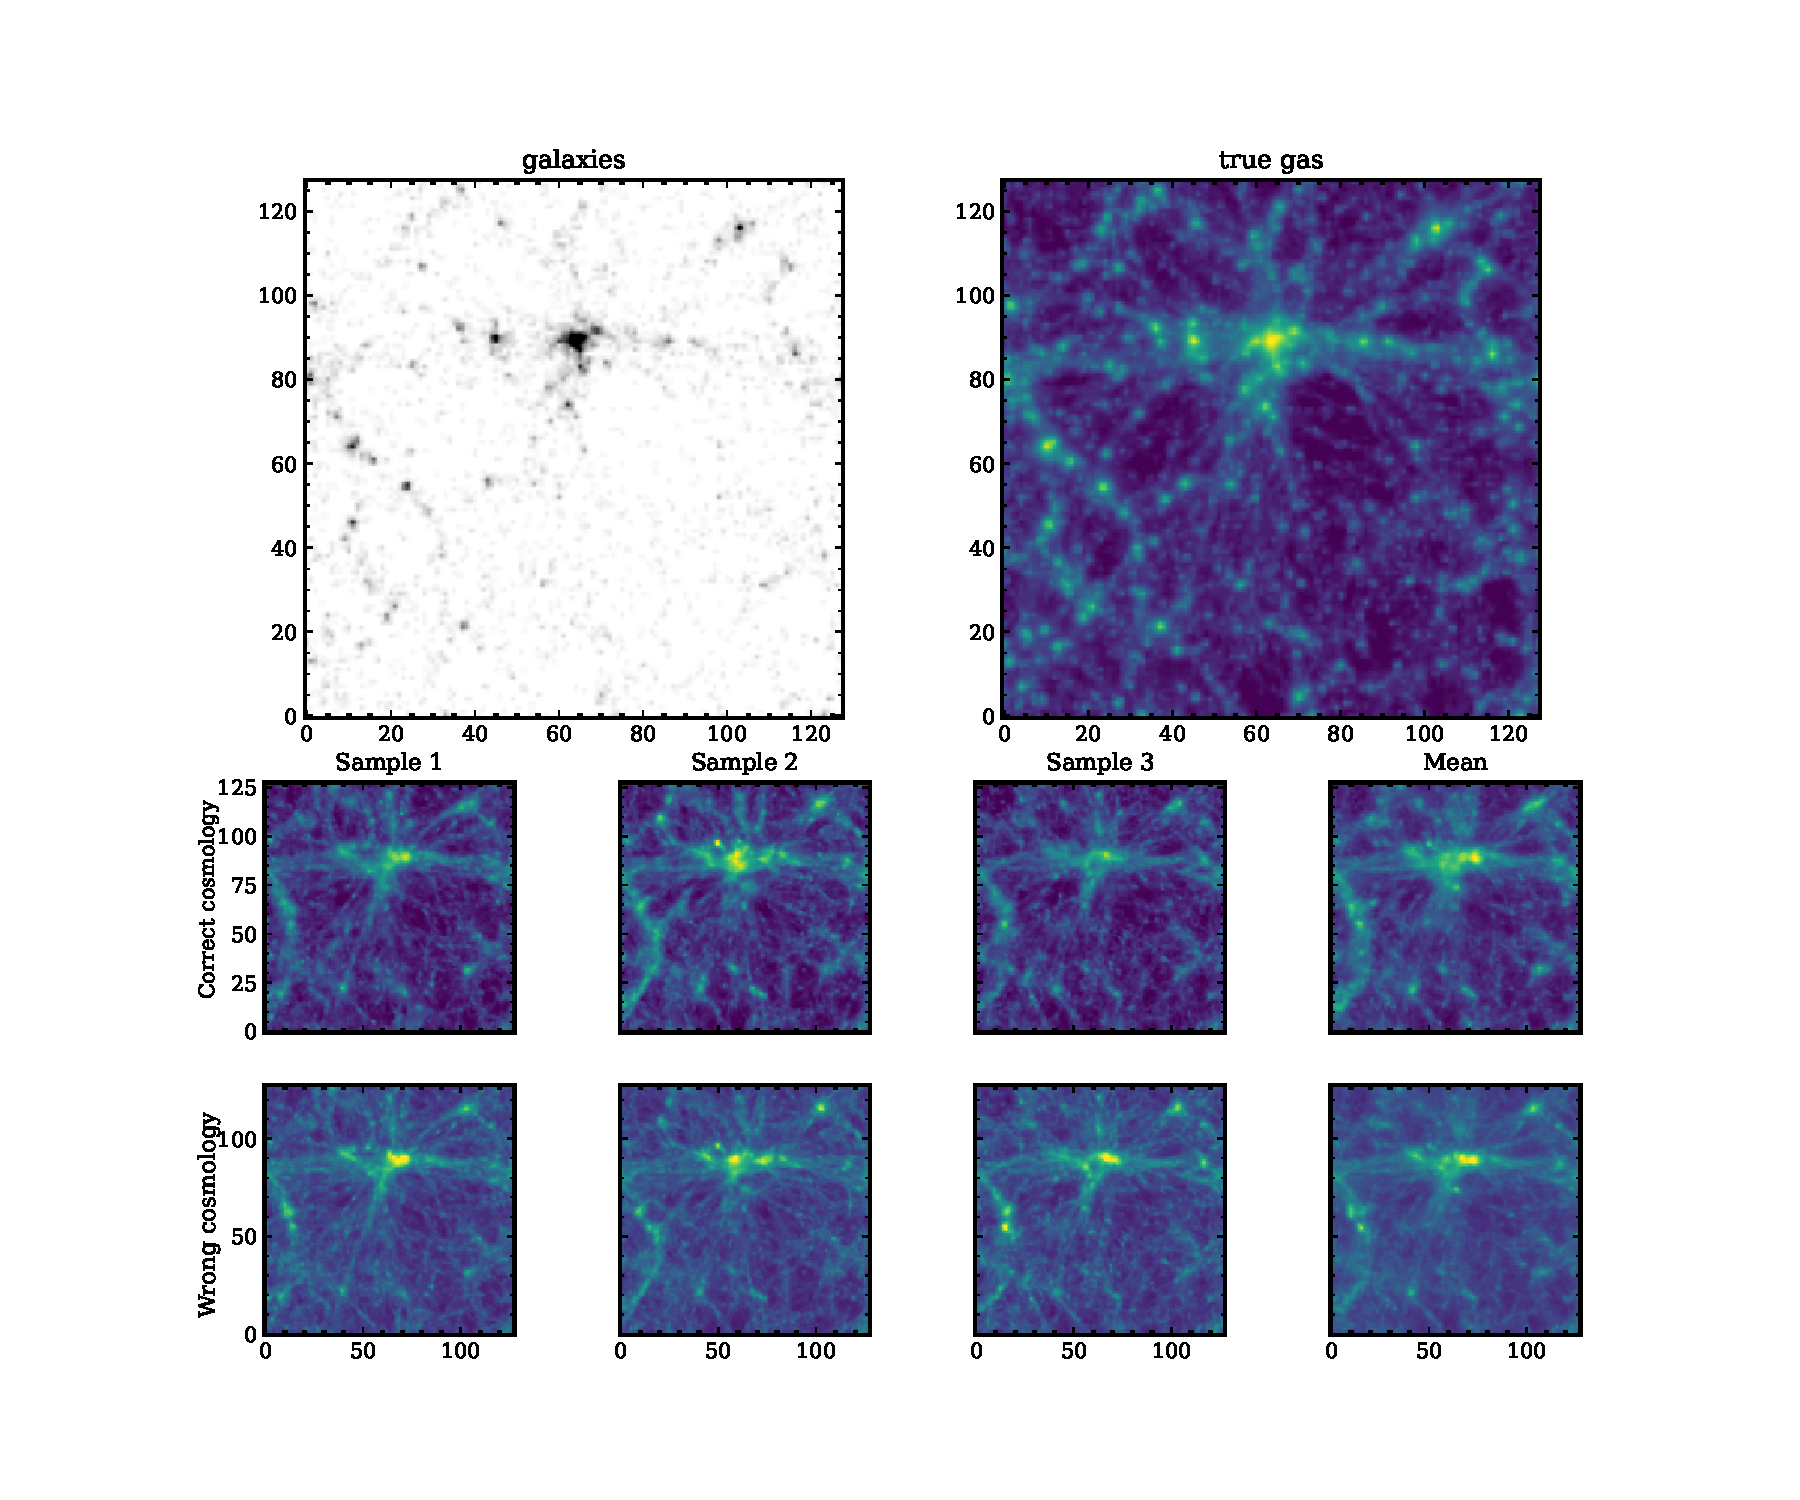
\includegraphics[width=0.5\linewidth]{figures/correct_wrong_cosmology.pdf}
    \caption{\textbf{Top left:} Input galaxy density field used to condition the model. 
\textbf{Top right:} True gas density from the CAMELS50 simulation for this test box. 
\textbf{Middle row:} Three samples and the mean posterior of gas density when the model is conditioned on the same cosmological parameters as the test box; the predictions closely match the true gas distribution. 
\textbf{Bottom row:} Three samples and the mean posterior of gas density when the model is conditioned on an alternative cosmology; the predicted gas distribution shows reduced total gas content, consistent with a lower baryon universe as dictated by the parameters. 
This figure demonstrates that the diffusion model learns the relationship between cosmological parameters and gas distributions, producing physically plausible predictions that vary appropriately with input parameters.}
    \label{fig:1}
\end{figure}

\begin{figure}
    \centering
    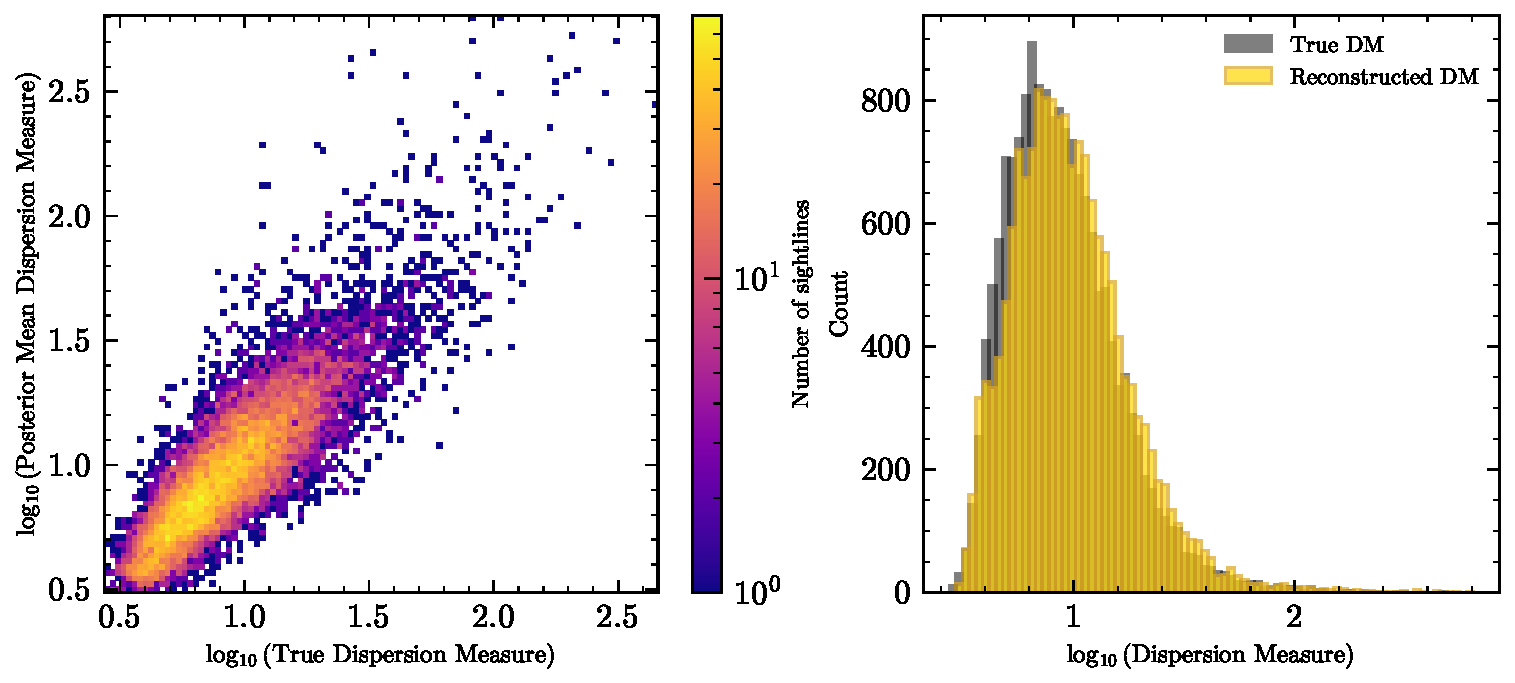
\includegraphics[width=0.5\linewidth]{figures/DM_recon_DM_true.pdf}
    \caption{box 10. }
    \label{fig:placeholder}
\end{figure}



\begin{figure}
    \centering
    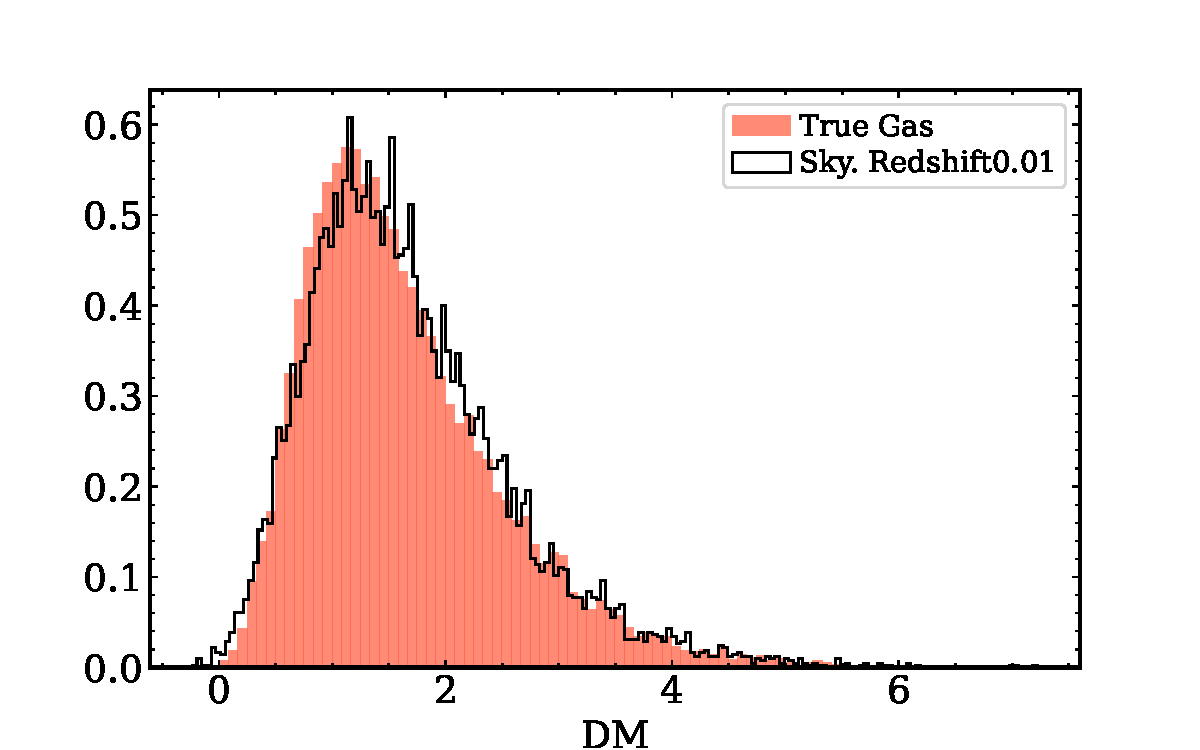
\includegraphics[width=0.5\linewidth]{figures/all_sky.pdf}
    \caption{Comparison of dispersion measure (DM) distributions from a CAMELS50 reconstruction field and TNG simulated FRBS. The red histogram shows the dispersion measure (DM) distribution calculated by integrating the gas density along all lines of sight through a CAMELS50 simulation box of size $50\,h^{-1}\,\mathrm{Mpc}$. The black histogram shows the DM distribution from 1000 randomly placed FRBs at a distance of 50 Mpc in the TNG50 simulation, corresponding to the path length through a CAMELS50 box. The reconstructed gas distributions produce DM values consistent with TNG FRB dispersion measures.\textbf{xxx wait, are we saying CAMELS recon distribution matches TNG random FRB DMs? what does that prove?}
}
    \label{fig:placeholder}
\end{figure}

\begin{figure}
    \centering
    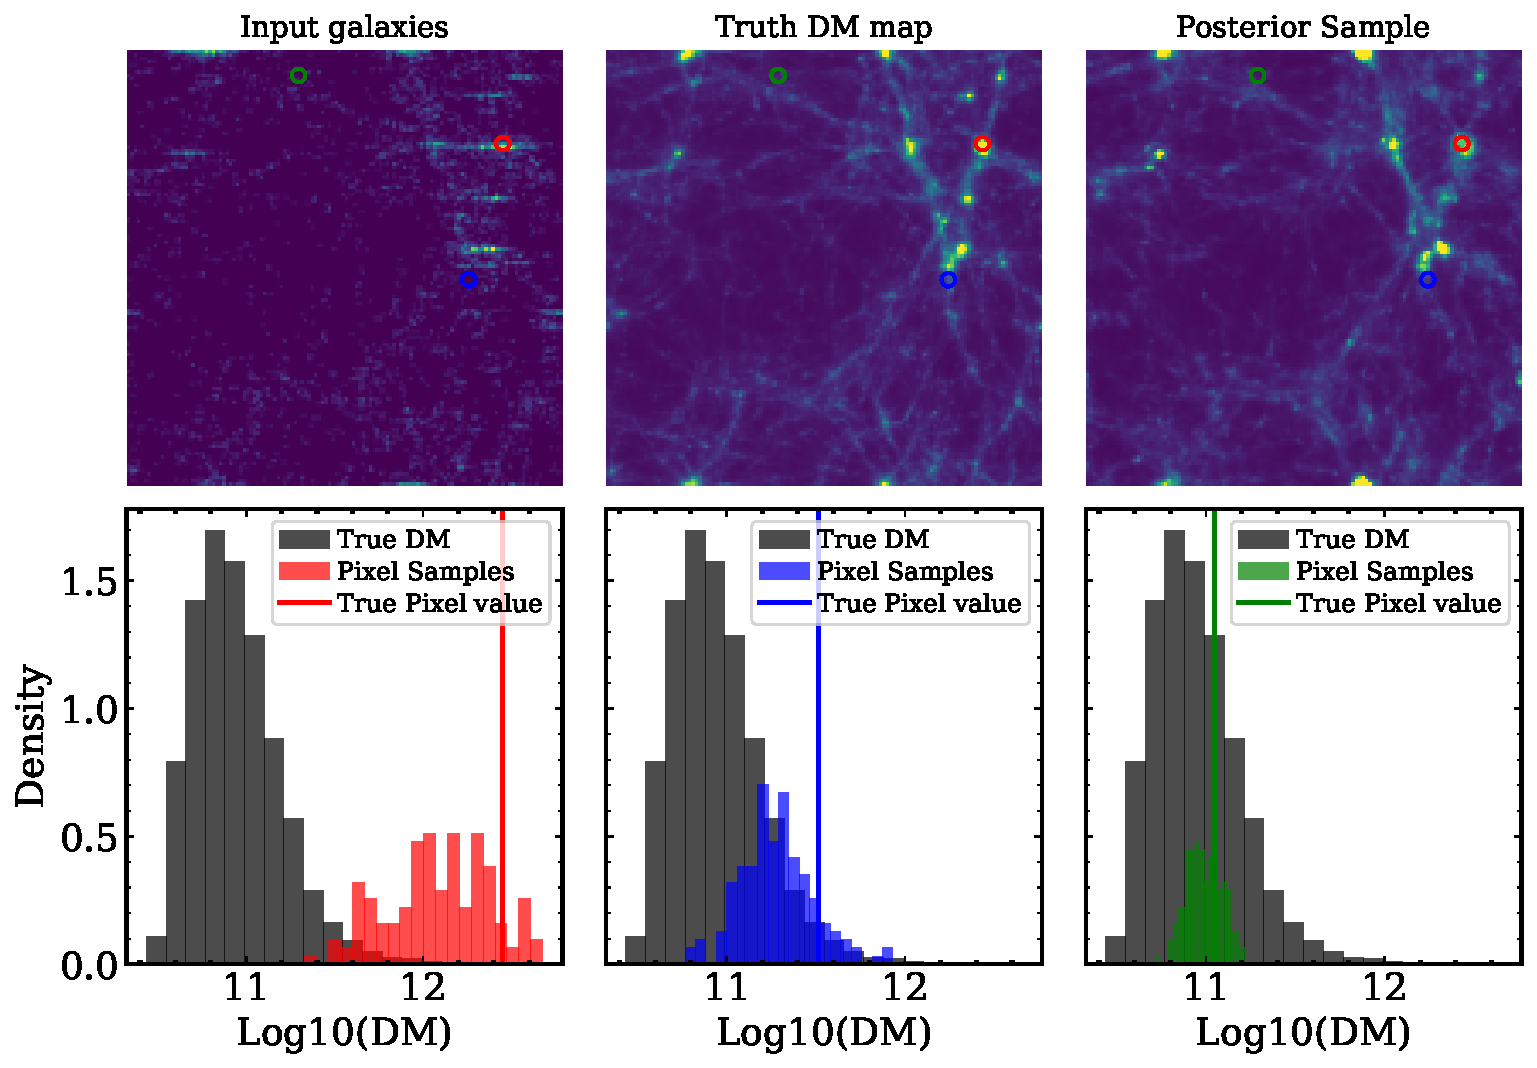
\includegraphics[width=0.5\linewidth]{figures/patch_hist_box9.pdf}
    \caption{Distribution of dispersion measure values for test box 9 in CAMELS. The black histogram shows the distributions of true DM values across the entire box. The black vertical line marks the true value of a single pixel, and the black histogram shows the distribution of that pixel's value across 150 different samples. This comparison shows that the model's samples recover a distribution centered near the true pixel value, consistent with a normal distribution around the ground truth.}
    \label{fig:placeholder}
\end{figure}

\section{Methods}
\label{sec:methods}
In this work we use 3D maps from CAMELS50 to model the connection between galaxy field and gas. We use the IllustrisTNG suite. CAMELS simulations have a box volume of $(50\,h^{-1}\,\mathrm{Mpc})^3$. We used 1000 simulation boxes with dimensions $50 \times 50 \times 50\,(\,h^{-1}\,\mathrm{Mpc})^3$ that included the parameters for that box, 3D galaxy density weighted by stellar mass, and gas 3D density. Each box is 128 x 128 x 128 pixels. 

Since TNG50 has a box size of $(35\,h^{-1}\,\mathrm{Mpc})^3$, which differs from the CAMELS50 training data at $(50\,h^{-1}\,\mathrm{Mpc})^3$, we needed to rescale the TNG50 data to match the model's training distribution. The volume difference results in different pixel sizes and galaxy number densities per voxel.

We preprocessed the TNG50 data as follows:
\begin{enumerate}
    \item Rescaled all galaxy positions by a factor of $\frac{50}{35}$ to map them into the CAMELS50 box size.
    \item Created a $128^3$ voxel grid spanning the rescaled $50\,h^{-1}\,\mathrm{Mpc}$ box.
    \item Applied a minimum stellar mass threshold, removing all galaxies with $M_{\star} < M_{\star,\mathrm{min}}$.
    \item Populated the grid using Cloud-In-Cell (CIC) interpolation, weighting each galaxy by $\log_{10}(M_{\star})$, where $M_{\star}$ is stellar mass.
    \item Computed $\log_{10}$ of the resulting density field.
    \item Normalized using the mean and standard deviation from CAMELS50 training: 
    $\tilde{f}_{\mathrm{gal}} = \frac{\log_{10}(f_{\mathrm{gal}}) - \mu}{\sigma}$, 
    where $\mu = \text{XXX}$ and $\sigma = \text{XXX}$.
\end{enumerate}
\section{Simulation}
\label{sec:data}
% \begin{figure}
%     \centering
%     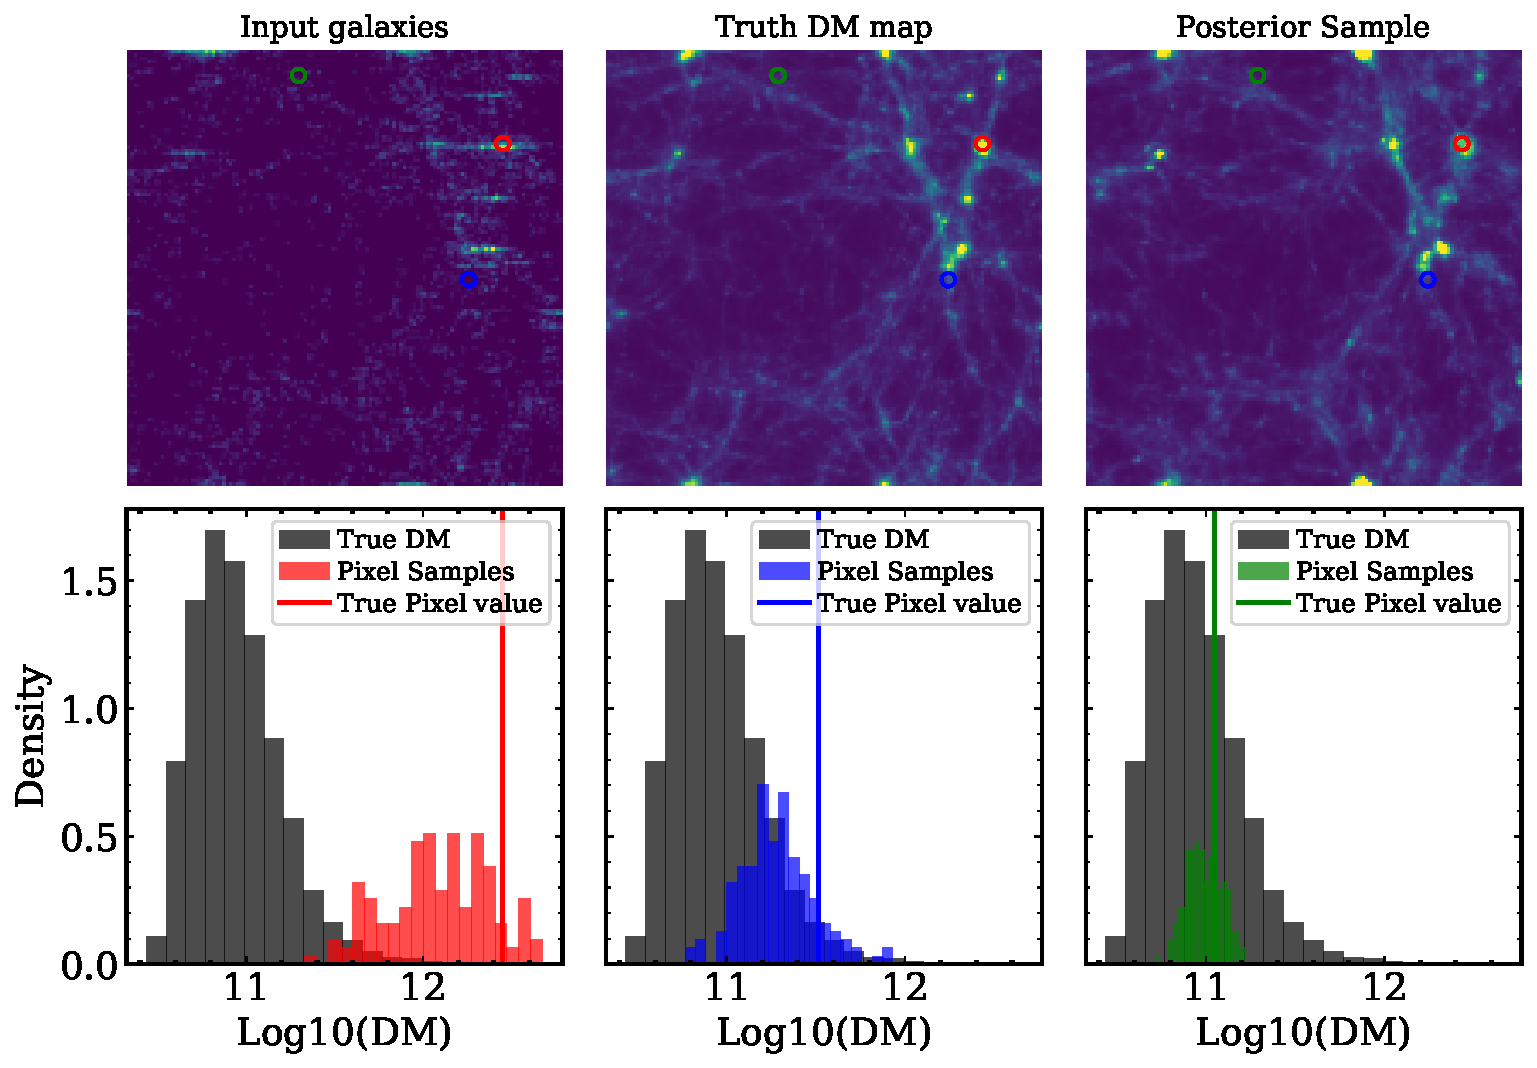
\includegraphics[width=0.5\linewidth]{figures/patch_hist_box9.pdf}
%     \caption{Caption}
%     \label{fig:placeholder}
% \end{figure}
\section{Results}
\label{sec:results}
we give the model a galaxy field a set of parameters. Ideally, the model will know how to map the galaxy field into a gas distribution in a way that preserve the constrains set by the parameters. So, for the same galaxy field input and the same seed, if $\Omega_b$ is higher we would expect more gas. Testing this hypothesis, that’s what we see in figure \ref{fig:1}. The right cosmology row refers to a set of parameters that have the same values as the test box, so the gas distribution we get should match that of the test box. The wrong cosmology row has lower value cosmological parameters than what we have in the test box, so the gas distribution should be a little more sparse and have less gas in total. 
\section{Discussion}
\label{sec:discussion}

\section{ACKNOWLEDGMENTS}

\clearpage

\bibliography{ref}
\end{document}
